\documentclass[english,11pt,]{article}
\usepackage{lmodern}
\usepackage{amssymb,amsthm,amsmath,wasysym}
\usepackage[nottoc]{tocbibind}
\usepackage{stmaryrd}
\usepackage{xspace}
\usepackage{ifxetex, ifluatex}
\usepackage[T1]{fontenc}
\usepackage{multirow}



\PassOptionsToPackage{usenames,dvipsnames}{xcolor}
\usepackage{beamerarticle}
%\usepackage[usenames,dvipsnamesnames]{xcolor}
\definecolor{gris}{rgb}{0.9,0.9,0.9}


\ifxetex
  \usepackage{polyglossia}
  \setmainlanguage{english}
\else
  \usepackage[utf8]{inputenc}
  \usepackage[shorthands=off,english]{babel}
\fi

% use upquote if available, for straight quotes in verbatim environments
\IfFileExists{upquote.sty}{\usepackage{upquote}}{}
% use microtype if available
%\IfFileExists{microtype.sty}{%
%\usepackage[babel=true,kerning=true]{microtype}
%\UseMicrotypeSet[protrusion]{basicmath} % disable protrusion for tt fonts
%}{}


\usepackage[margin=2.5cm]{geometry}


\usepackage{csquotes}

\setcounter{tocdepth}{3}

%\usepackage[natbib=true, backend=bibtex, bibstyle=authoryear, citestyle=authoryear-comp, url=false, doi=false]{biblatex}
\usepackage[natbib=true, backend=bibtex, url=false, doi=false]{biblatex}
		\bibliography{../publis.bib,../974.bib}
	

\usepackage{longtable,booktabs}

\usepackage{graphicx}
  
\usepackage{subfig}




%
\makeatletter
\def\maxwidth{\ifdim\Gin@nat@width>\linewidth\linewidth\else\Gin@nat@width\fi}
\def\maxheight{\ifdim\Gin@nat@height>\textheight\textheight\else\Gin@nat@height\fi}
\makeatother
% Scale images if necessary, so that they will not overflow the page
% margins by default, and it is still possible to overwrite the defaults
% using explicit options in \includegraphics[width, height, ...]{}
\setkeys{Gin}{width=\maxwidth,height=\maxheight,keepaspectratio}

\ifxetex
	\usepackage[setpagesize=false, % page size defined by xetex
              unicode=false, % unicode breaks when used with xetex
              xetex]{hyperref}
\else
  \usepackage[unicode=true]{hyperref}
\fi
\hypersetup{breaklinks=true,
            pdfauthor={Flores O.},
            pdftitle={Bird community assembly along an elevation profile on a remote tropical volcanic island},
            colorlinks=true,
            citecolor=blue,
            urlcolor=blue,
            linkcolor=blue,
            pdfborder={0 0 0}}
						
\urlstyle{same}  % don't use monospace font for urls
%\setlength{\parindent}{0pt}
\setlength{\parskip}{8pt plus 2pt minus 1pt}
\setlength{\emergencystretch}{3em}  % prevent overfull lines
\setcounter{secnumdepth}{3}



%%% Change title format to be more compact
\usepackage{titling}
%\setlength{\droptitle}{-2em}


\title{Bird community assembly along an elevation profile on a remote tropical
volcanic island}


    \usepackage{authblk}
                                        \author{Flores O.}
                        
  \date{}
%  \predate{}\postdate{}


\definecolor{fgcolor}{rgb}{0, 0, 0}
\newcommand{\hlnum}[1]{\textcolor[rgb]{0.565,0.439,0}{#1}}%
\newcommand{\hlstr}[1]{\textcolor[rgb]{0,0.439,0.408}{#1}}%
\newcommand{\hlcom}[1]{\textcolor[rgb]{0.376,0.376,0}{#1}}%
\newcommand{\hlopt}[1]{\textcolor[rgb]{0,0,0}{#1}}%
\newcommand{\hlstd}[1]{\textcolor[rgb]{0,0,0}{#1}}%
\newcommand{\hlkwa}[1]{\textcolor[rgb]{0.125,0.376,0.659}{#1}}%
\newcommand{\hlkwb}[1]{\textcolor[rgb]{0.031,0.314,0.627}{#1}}%
\newcommand{\hlkwc}[1]{\textcolor[rgb]{0.659,0.412,0.125}{#1}}%
\newcommand{\hlkwd}[1]{\textcolor[rgb]{0.125,0.659,0.145}{#1}}%

\usepackage{framed}
\makeatletter
\newenvironment{kframe}{%
 \def\at@end@of@kframe{}%
 \ifinner\ifhmode%
  \def\at@end@of@kframe{\end{minipage}}%
  \begin{minipage}{\columnwidth}%
 \fi\fi%
 \def\FrameCommand##1{\hskip\@totalleftmargin \hskip-\fboxsep
 \colorbox{shadecolor}{##1}\hskip-\fboxsep
     % There is no \\@totalrightmargin, so:
     \hskip-\linewidth \hskip-\@totalleftmargin \hskip\columnwidth}%
 \MakeFramed {\advance\hsize-\width
   \@totalleftmargin\z@ \linewidth\hsize
   \@setminipage}}%
 {\par\unskip\endMakeFramed%
 \at@end@of@kframe}
\makeatother

\definecolor{shadecolor}{rgb}{.95, .95, .95}
\definecolor{messagecolor}{rgb}{0, 0, 0}
\definecolor{warningcolor}{rgb}{1, 0, 1}
\definecolor{errorcolor}{rgb}{1, 0, 0}
\newenvironment{knitrout}{}{} % an empty environment to be redefined in TeX

\renewenvironment{knitrout}{\renewcommand{\baselinestretch}{0.8}}{}
%%%%%%%%%%%%%%%%%%%%%%%%
%\PassOptionsToPackage{dvipsnames}{color}
%\usepackage[dvipsnames]{xcolor}
%\definecolor{gris}{rgb}{0.9,0.9,0.9}
%\definecolor{cerulean}{rgb}{0.0, 0.48, 0.65}
%\definecolor{cadet}{rgb}{0.33, 0.41, 0.47}

\usepackage{thmtools}
\mode<article>{\declaretheorem[shaded={bgcolor=gris!80!white, textwidth=\textwidth}, name=Définition]{defn}
\renewcommand{\listtheoremname}{Liste de définitions}}
\mode<beamer>{\declaretheorem[name=Définition]{defn}}

%\newenvironment<>{exemple}[1]{%
%  \setbeamercolor{block title}{fg=white,bg=red!75!black}%
%  \begin{block}#2{#1}}{\end{block}}


%%\newcommand{\tightlist}{\setlength{\itemsep}{0pt}\setlength{\parskip}{0pt}}
%\newcommand\malt[2]{\mode<article>{#1}	\mode<beamer>{#2}}
%\newcommand\code[1]{\textsf{\textbf{#1}}}
%\renewcommand\belowcaptionskip{2ex}
%\newcommand\mart[1]{\mode<article>{#1}}
%\newcommand\mbea[1]{\mode<beamer>{#1}}

\newcommand*\chem[1]{\ensuremath{\mathrm{#1}}}

\def\chaptername{Partie}

\renewcommand\keywords[1]{\textbf{Keywords:} #1}


\usepackage{alltt}
\usepackage{multirow}


\graphicspath{{../figures/}}

    ../../../code/TeX/especes.tex
    ../../../code/TeX/newcom.tex
  
\newenvironment<>{exemple}[1][]{%
  \setbeamercolor{block title example}{fg=white,bg=structure.fg!95!blue}%
  \begin{example}#2[#1]}{\end{example}}



\newcommand{\tightlist}{\setlength{\itemsep}{0.7pt}\setlength{\parskip}{0.7pt}}

%----- DOC BEGINS ----------------------------------------------

\begin{document}

\maketitle


\begin{abstract}
\hrule
\medskip
Although biological invasions are one of the most important changes in
ecological dynamic, they have been rarely investigated along elevational
gradients. The objective of this study was to compare the distributions
of exotic versus native birds on a same broad elevational gradient.
Field studies were conducted on the leeward side of Reunion Island
(Mascarene Archipelago, Western Indian Ocean) between 20 and 2880 m at
363 sampling points. Species richness and abundances of bird species
were surveyed during the nesting season using 20 min count at each
point. Mean elevational position and elevational amplitude were measured
for each species and a Mean Distribution Index was computed as the
number of bird species having their mean elevation within each 100 m
elevational band. The data show that (1) the elevational variation of
native species richness is hump-shaped, whereas the richness of exotic
bird species does not vary in the first half of the gradient; (2) the
elevational amplitude and maximum elevation do not differ significantly
between exotic and native birds, but the mean and minimum elevations are
higher for native birds; and (3) the most suitable vegetation types are
found in the `rural landscapes' belt for the exotic bird communities,
and in the higher belt of `forest and pastures' for the native ones.
Even if history can appear too short to permit niche expansion of the
more recent introduced species, we can underline the exotic species
preference for anthropogenic landscapes and their large amplitude in
elevation.
\end{abstract}



\hrule

{\hypersetup{linkcolor=black}

%--------list of definitions ----------
}



The conspicuous ecological changes that occur along elevational
gradients have drawn the attention of an increasing number of studies.
Most hypotheses which attempted to explain biological responses to
elevational gradients were formally based on a single bio-physical
factor such as productivity, habitat diversity, environmental stress,
resource availability or competition (e.g.~Rahbek, 1995; Heaney, 2001).
Others underlined the role of anthropogenic pressure or ecological and
evolutionary processes (e.g.~Myers \& Giller, 1988).

Surprisingly, studies on species distribution along elevational
gradients scarcely pay attention to the status of the involved species,
i.e.~either exotic or native, despite of the increased importance of the
impact of introduced species on biodiversity (Vitousek et al., 1997).
The same can be said of studies on latitudinal gradients (but see Sax,
2001). Considering the theoretical framework of biological invasions,
investigations on the distribution of exotic species along broad
ecological gradients should enable us to predict invasion patterns.

Birds, widely introduced throughout the world and having colonized most
vegetation types (Long, 1981), are a relevant taxon for studying the
comparative distribution of exotic versus native species along
elevational gradients. Exotics are species that have been introduced by
humans, or have been able to expand their range because of anthropogenic
disturbances, into geographical regions in which they were not
historically present (Sax, 2001). Birds have been widely used as models
in studies on the variation of species richness with elevation
(Thiollay, 1980; Patterson et al., 1998; Benning et al., 2002 ; Prodon
et al., 2002). The elevational range of bird communities is also of
special interest as it is one of the dimensions of the niche of a
species, and it is linked to flexibility in habitat or food choices,
ability to coexist with different species, and physiological tolerance
(Prodon et al., 2002). \% Last, the mean elevational position can be
considered to be an indicator for determining one of the optimal
vegetation types of a species.

In this paper, we use past data to document the elevational patterns of
bird assemblages on a tropical volcanic island. We specifically adress
the question whether elevational distribution patterns differ between
exotic and native bird species. We analyse patterns along a slope on
Reunion Island (Indian Ocean) that presents one of the widest
bio-climatic gradients within any oceanic island, \textit{i.e.} from 0
to more than 3000 m on a distance of 20 km. We first characterize
species distribution along the gradient and compare distribution
parameters across native and exotic species. We then characterize
patterns of species richness and compare the observed patterns to two
different nul models.

Analysing observed patterns relatively to nul models expectations can
inform on assembly processes. Nul models differ in the way they assemble
community data, that is species occurrence data, here abundance, in
sampled sites. They can include several constraints which consist in
preserving some properties of the observed data, such as species overall
abundance or local abundance at each sampled site. Here, the two tested
models assemble species randomly preserving their frequency along the
gradient, in order to retain differences in rarity. The first model is
constrained by the total abundance of birds observed locally that is
held constant during estimation. The model thus conserves interactions
between total abundance and the environment, which can be referred to as
the \enquote{site capacity hypothesis}.

This capacity is supposed to be mobilized by birds present to some
constant level, which is reflected in the total estimated abundance.

In the second model, these interactions are suppressed supposing that
site capacity varies randomly. In this model, the sites are supposed as
equal in their capacity to support birds to some random level.

Comparing observed data with nul models allows to explore differences in
the elevational patterns of species richness between native and exotic
birds under the constraint of observed commonness and site capacity or
not.

\section{Material and methods}\label{material-and-methods}

\subsection{Studied area}\label{studied-area}

Reunion Island is part of the Mascarene volcanic archipelago, situated
in the Western Indian Ocean (55°30' E and 21°05' S)(Fig. 1). This
oceanic island appeared three million years ago. In the centre of the
island, a plateau (Plaine des Caffres, \(\approx\) 2000 m) is flanked by
two volcanoes (Piton de la Fournaise, 2631 m; Piton des Neiges, 3069 m),
the sides of which slope steeply towards the sea. There is a very steep
climatic gradient: the average minimum ground temperature falls below
0°C above 1500 m in August, above 1800 m from June to October, and above
2300 m all year round; at the highest point, the temperature ranges from
-10°C to +26°C \autocites{Cadet1974}{Raunet1991}. The studied area,
located on the leeward side of the island had a slope of about 0.15 m
per m and an annual rainfall ranging from 500 mm at sea level to 2000 mm
on the highest mountain slopes \autocite{Raunet1991}. The land is
roughly organized through a land use gradient into a succession of
elevational belts \autocite{cadet_vegetation_1980} urbanised areas (0-50
m a.s.l.), herbaceous savannah (50-300 m), sugarcane monoculture
(300-800 m), rural landscapes with diversified crops (800-1200 m),
primary forest mixed with pastures and planted forests (1200-1800 m),
heathlands dominated by ericaceous plants (1800-2600 m), and bare soils
with a very sparse vegetation of herbaceous species (2600-3069 m) (Fig.
??). Above 1200 m, about 60 \ldots{}

\subsection{Sampling}\label{sampling}

The transect was sampled through one survey during the breeding season
(December, 1997 - April, 1998), using 363 sample points spread along an
elevational gradient from 20 m to 2880 m (Fig. ??). Further prospecting
between 2880 and 3069 m (Piton des Neiges) revealed no bird presence.
Sea birds nest at these high altitudes but were not considered in the
study. This was due to of a lack of vegetation, except for scarce
amounts of native herbs and weeds. Sampling points were equally
distributed all along the elevational gradient, with a mean elevational
distance of 8 m between two successive elevations, and a distance of at
least 250 m between two successive count points, a mean sampling
pressure of 12.7 count points per 100 m elevational band, and covering
the overall diversity of vegetation types. Depressions, ridges and mires
were avoided in order to avoid extremely wet or dry places. We also
avoided places too close to feeding troughs in grasslands as they
attract granivorous bird species. We assume that most of the birds were
sampled near their nesting sites. In order to limit sampling bias, the
different ecosystems found at each 100~m elevational band were surveyed
so as not to miss individual bird species specific to individual
ecosystems.

\subsection{Data analysis}\label{data-analysis}

We calculated the weighted mid-point of species distribution as the
average of all elevations where a species was detected weighted by the
number of times it was detected. We also compare species maximal and
minimal elevation where observed along the gradient, and amplitude in
elevation range. We use the word elevation instead of altitude, as
elevation is meters above sea level where altitude is meters above
ground.

We compared observed species richness in the two groups of bird species
(native and exotic) to two different nul models based on random
permutations of the original dataset \autocite{Gotelli2000}. In both
models, species overall abundance, that is the total number of records
for each species, was preserved in each permutation, in order to account
for observed differences in species commonness and detectability. The
main difference between the two nul models was in the treatment of site
carrying capacity of birds diversity, which under equilibrium hypothesis
can be estimated as the total numbers of individuals locally. In the
first nul model (N1), sites are considered as equally suitable for
birds. In this case, the randomization suppresses any structure that
exists in the data due to relationships between carying capacity and
environment (here elevation) in a broad sense. The randomized pattern
obtained mimics the distribution of species richness not accounting for
those relationships. In the second nul model (N2), the carying capacity
of sites, that is local species richness, was preserved by the
randomization procedure. This model holds account for differences in
sites to support bird abundance in relation with habitat carrying
capacity. In this case, the randomized pattern obtained takes into
account both species commonness and site suitability. The total number
of individuals observed locally is preserved and species abundance in
the dataset are preserved, but individuals and samples are randomized
across sites. For each model, we performed a number of permutations
(\(n=1999\)) to obtain 95-\% confidence intervals on simulated species
richness. \# Results

Twenty-two bird species were recorded over the 363 sampling points, with
a mean of species per point and species per 100-m elevational band along
the gradient. Fourteen species were exotic and eight native
tbl.~\ref{tbl:species}. The number of records varied widely across
species between 1 for two species (\emph{,} ) and 268 for ** (mean:
\(\pm\) s.d.: , Fig. \[boxalti\]).

Amplitudes in elevational range were high. Elevational amplitude
exceeded 2000~m for five species and 1000~m for 15 species (Table 1).
The largest elevational amplitude measured in native species was for
\emph{Zosterops borbonicus} (92 \% of the gradient) and for
\emph{Acridotheres tristis} in exotic species (83 \%) . The lowest
elevational amplitude measured in native species was registered for
\emph{Circus maillardi} (20 \%) and for \emph{Perdicula asiatica} in
exotic species (8 \%). The distribution of weighted mid-points, that is
the weighted mean of elevations where a species occurs along the
gradient, was highly concentrated between 1000 and 1500 m, with the
exception of three exotic species (Fig.~\ref{fig:boxrange}). The
weighted mid-point and minimum elevation were however higher in native
species (\(p=0.034\) and \(p=0.024\)). By contrast, elevational
amplitude and maximum elevation did not differ significantly between the
two groups of species (\(p=0.534\) and \(p=0.254\) respectively,
Fig.~\ref{fig:boxrange}). No difference in the variability of species
distribution was observed across the two groups: Bartlett test's of
variance homogeneity showed that the variability was similar in the two
groups for the four tested variables.

The total species richness observed within 100-m elevation bands varied
between 2 and 19 (10.4 \(\pm\) 5.5, Fig.~\ref{fig:Sgam}.a). Total
richness showed a unimodal mid-elevational peak between 1000 and 1200~m.
However, the pattern of species richness differed significantly between
exotic and native species with increasing elevation
(Fig.~\ref{fig:Sgam}). Species richness varied between 0 and 7 for
native birds (3.5 \(\pm\) 2.2), and between 1 and 12 (6.9 \(\pm\) 3.9)
for exotic birds (Fig.~\ref{fig:Sgam}.b). Species richness showed
different elevational patterns across the two groups. Species richness
of native birds showed a unimodal mid-elevational peak around 1200~m,
whereas richness for exotic birds species showed a low-elevation plateau
with a small mid-peak also around 1200~m. Exotic species were more
numerous than native birds up to mid-elevation, whereas native species
were more numerous at higher altitudes (Fig.~\ref{fig:Sgam}.b).
According to richness patterns, three zones could be defined: (1) from 0
to 900 m, there was a significant difference between exotic and native
species, both in the number of species contacted and in their variation
pattern, as native species increased with the elevational gradient from
two to seven while the exotic ones remained at a high level (around 9
species ); (2) from 1000 to 2000 m, richness of both exotic and native
species presented a peak (around 9 and 6 species, respectively); (3)
from 2000 to 3000~m, richness was higher in native species while exotic
species were barely present.

In order to explore species co-occurence according to their status, we
compared species richness to random patterns obtained by simulation.
Values occurring within the simulated 95\% confidence band for the
random pattern indicated elevation bands where species richness was not
statistically different from random patterns of species assemblage
Fig.~\ref{fig:Snul}. In both groups, null patterns showed higher
variability at low and high elevation when sites were all considered as
equally suitable (randomized total abundance), whereas null patterns
were more constrained when the total abundance observed at each site was
kept constant (site capacity hypothesis). All models showed
mid-elevation peaks however less pronounced under the site capacity
hypothesis.

Native species richness was significantly lower than random expectations
at low elevation for both null models (Fig.~\ref{fig:Snul}.a). This
finding indicates depauperate communities where native species occur
less frequently than expected by chance. From 900~m above, the observed
pattern in native species richness overall supported more the site
capacity hypothesis Regarding exotic birds, species richness was lower
than expected by chance above 1500~m high (Fig.~\ref{fig:Snul}.b). This
result indicates that exotic species in high elevation bird communities
are in low numbers compared to the site capacity. At low to mid
altitude, the observed pattern in exotic species richness was closer to
the confidence interval of the null model without constraint on site
capacity (equally suitable hypothesis). The site capacity hypothesis
generated higher than observed numbers of exotic species.

\section{Figure legends}\label{figure-legends}

Figure Fig.~\ref{fig:boxalti}: Box-and-whisker plots indicating the
median, first and third quartiles and values outside inter-quartile
range of elevations where species were detected. Species are sorted by
order of median evelation. Blue indicates native species, and red
indicate exotic species. Species are labelled with the first two letters
of the genus and species names (see Tbl.~\ref{tbl:species}).

Figure Fig.~\ref{fig:boxrange}: Four features of species distributions
with respect to elevation in native and exotic species : (a) weigthed
mid elevation point (average elevation where the species was detected
weighted by number occurences), (b) elevation amplitude (difference
between highest and lowest elevation of detection), (c) minimum
elevation where the species was detected and (d) maximal elevation of
detection. Box-and-whisker plots indicate the median, first and third
quartiles and values outside inter-equartile range. Symbols indicate
individual values (\(n=22\) species), open symbols indicate species with
less than 5 records in dataset (\(n=3\) species, see
Tbl.~\ref{tbl:era}).

Figure Fig.~\ref{fig:Sgam}: Elevation patterns of species richness : (a)
total and (b) according to species status, native or exotic. Richness is
calculated here per 100-m elevation band as the number of species
detected within the band. Dotted lines indicate generalized additive
models fits (GAM) with colored bands showing the 95\% confidence
interval on estimated richness.

Figure Fig.~\ref{fig:Snul}: Comparison between observed richness (dots)
within 100-m elevation bands for native (a. \& c.) and exotic (b. \& d.)
birds and expected species richness under two different null models that
simulate random species assemblages (95\%-confidence band). Green lines:
null model with fixed site capcity, blue lines: null model with random
site capacity (equally suitable sites hypothesis). In both models,
species frequencies in the dataset were preserved during simulation
(\(n=2000\)).

\newpage

\section{Figures}\label{figures}

\begin{figure}
\centering
\begin{tabular}{cc}
(a) & (b) \\

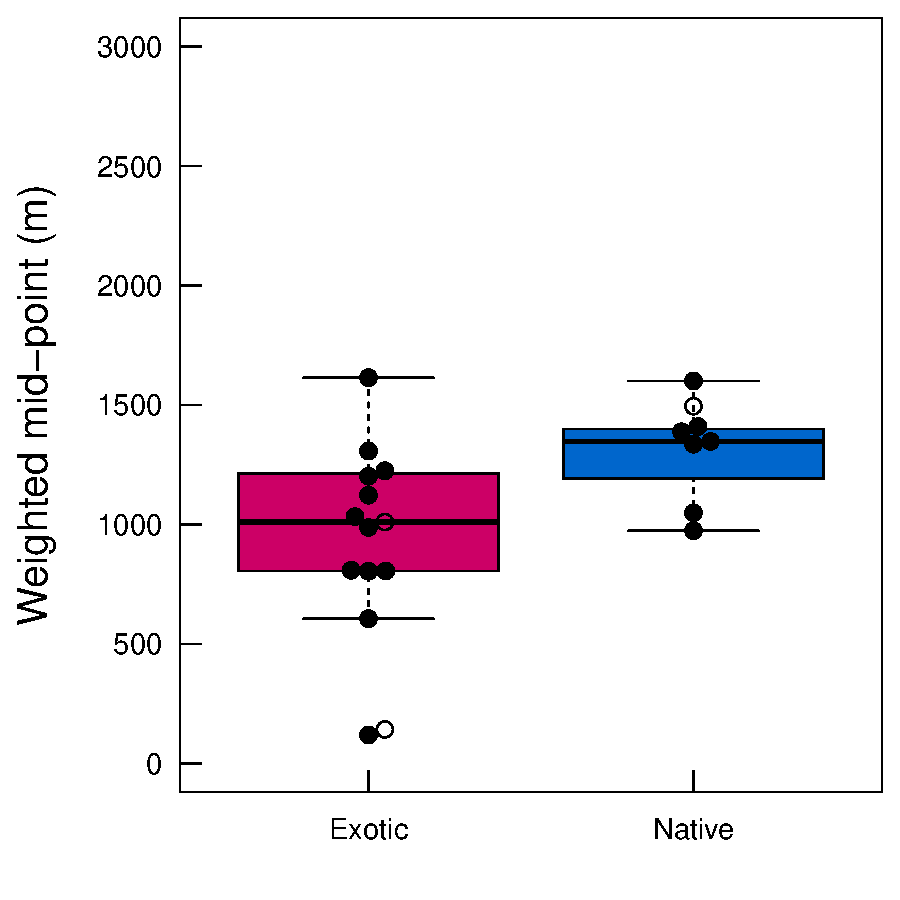
\includegraphics[width=0.5\textwidth]{../figures/div98-boxwmalt-1} 

&

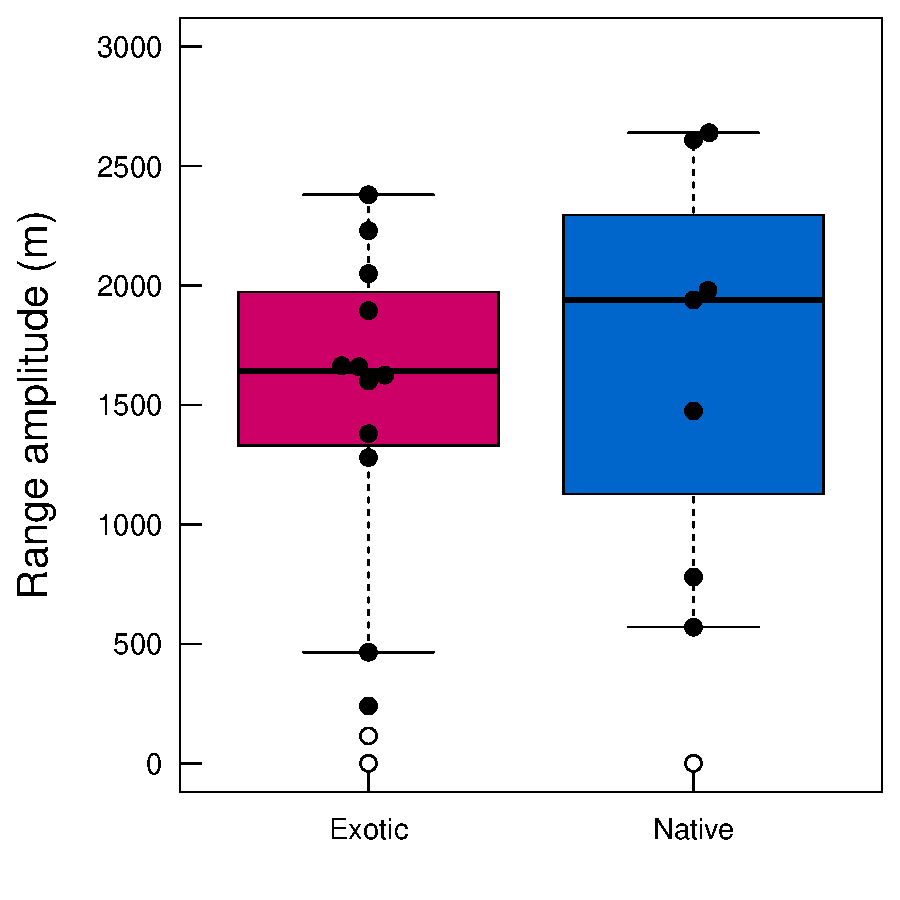
\includegraphics[width=0.5\textwidth]{../figures/div98-boxampl-1} 

\\
(c) & (d) \\

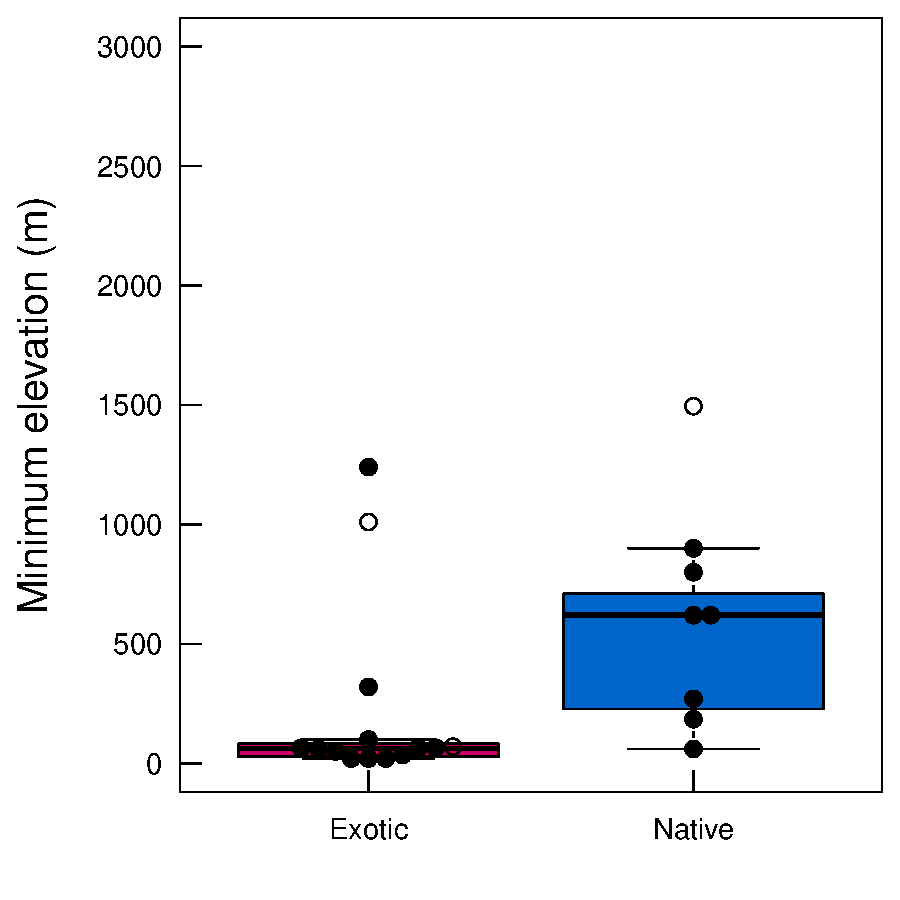
\includegraphics[width=0.5\textwidth]{../figures/div98-boxmin-1} 

&

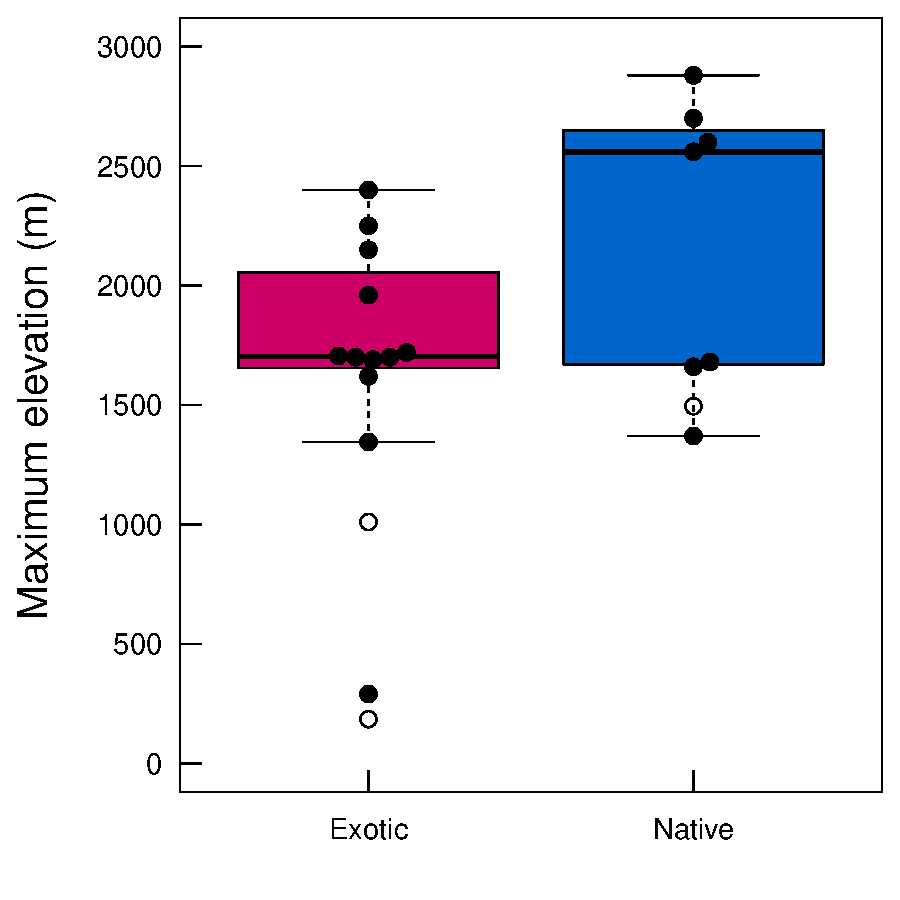
\includegraphics[width=0.5\textwidth]{../figures/div98-boxmax-1} 

\end{tabular}
\caption{\label{fig:boxrange}}
\end{figure}

\begin{figure}
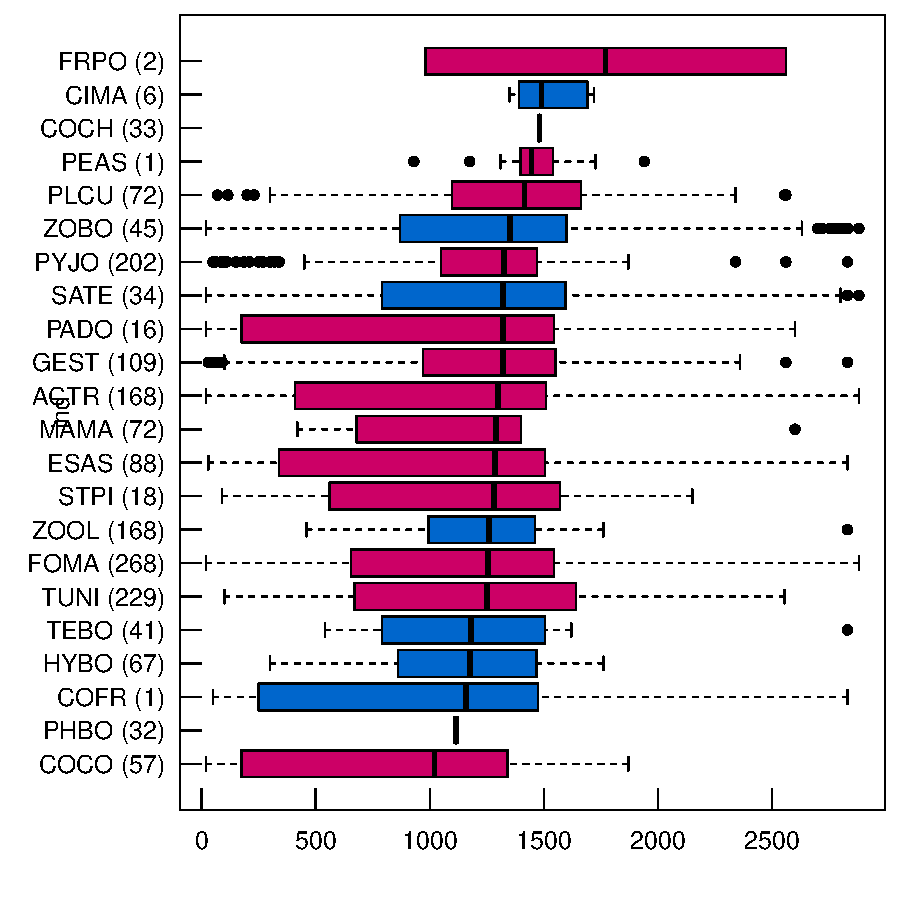
\includegraphics[width=\linewidth]{../figures/div98-boxalti-1} \caption{ }\label{fig:boxalti}
\end{figure}

\clearpage

\begin{figure}
\hspace{-2cm}
\begin{tabular}{cc}
a& b\\

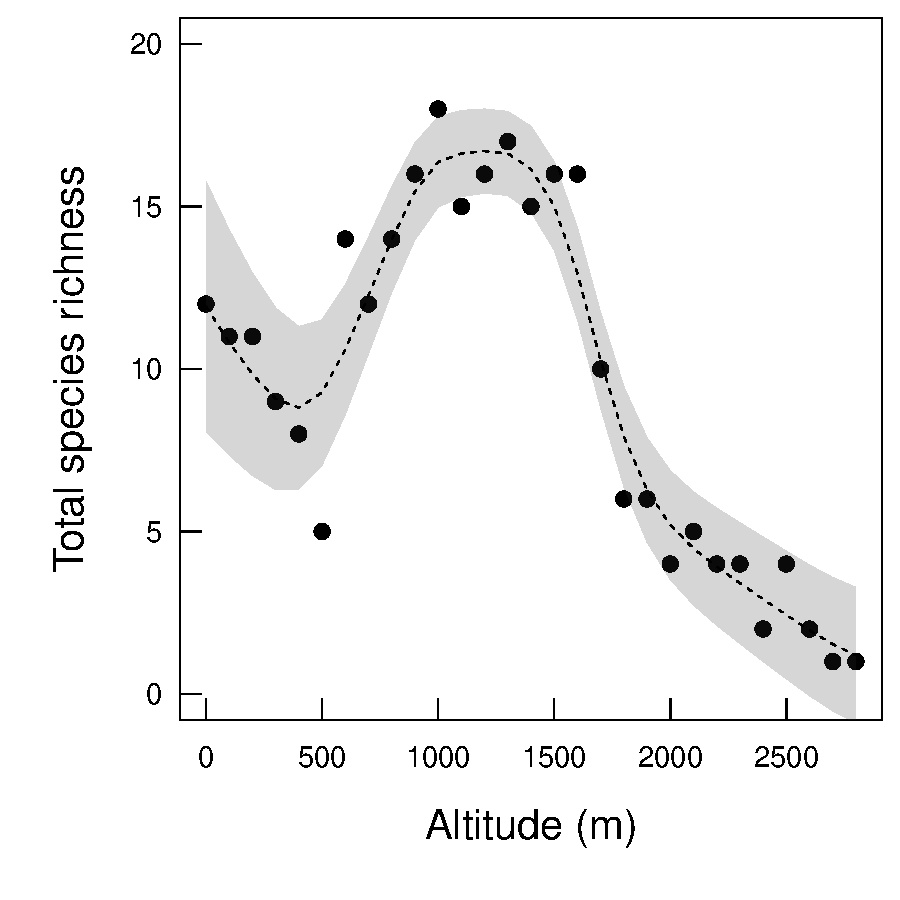
\includegraphics[width=0.5\linewidth]{../figures/div98-Stot-1} 
&

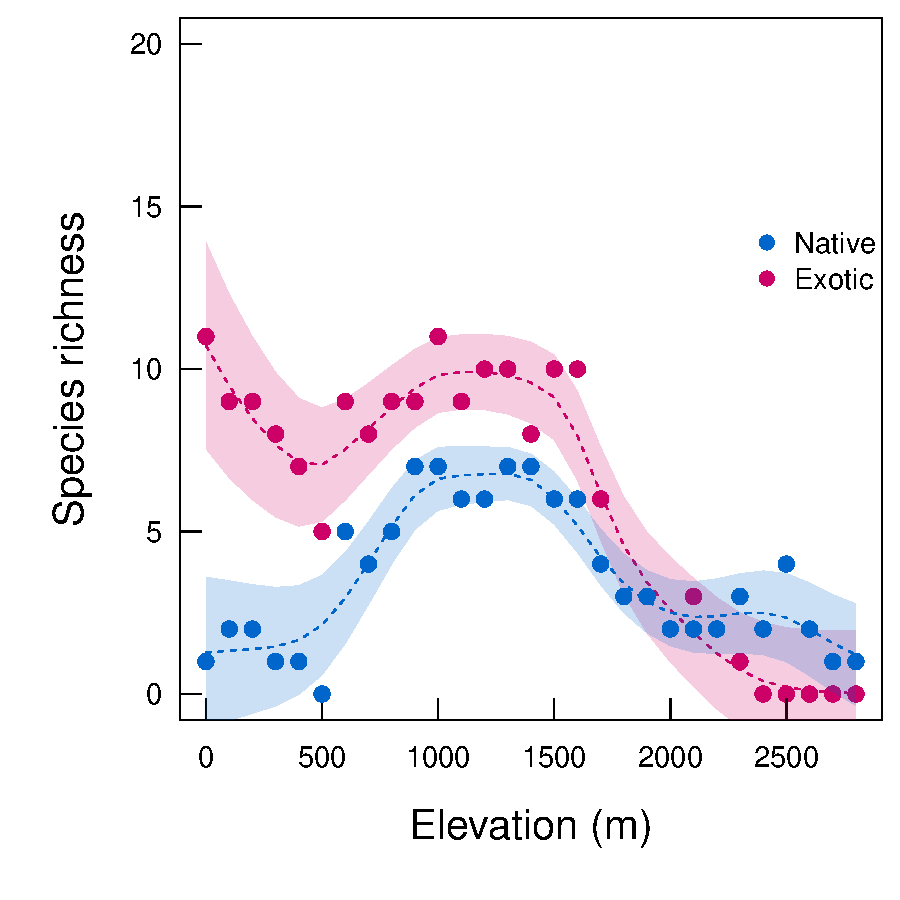
\includegraphics[width=0.5\linewidth]{../figures/div98-Snatexo-1} 

\end{tabular}
\caption{\label{fig:Sgam}}
\end{figure}

\clearpage

\begin{figure}
\hspace{-2cm}
\begin{tabular}{cc}

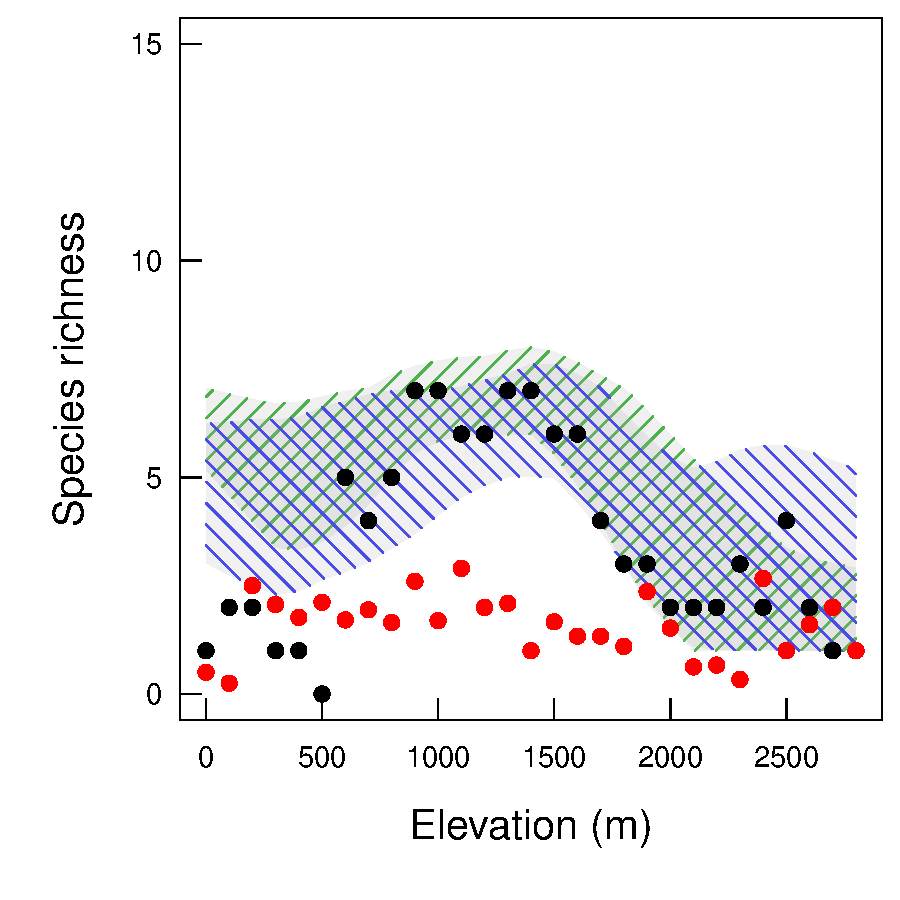
\includegraphics[width=0.5\linewidth]{../figures/div98-Snatnul-1} 

&

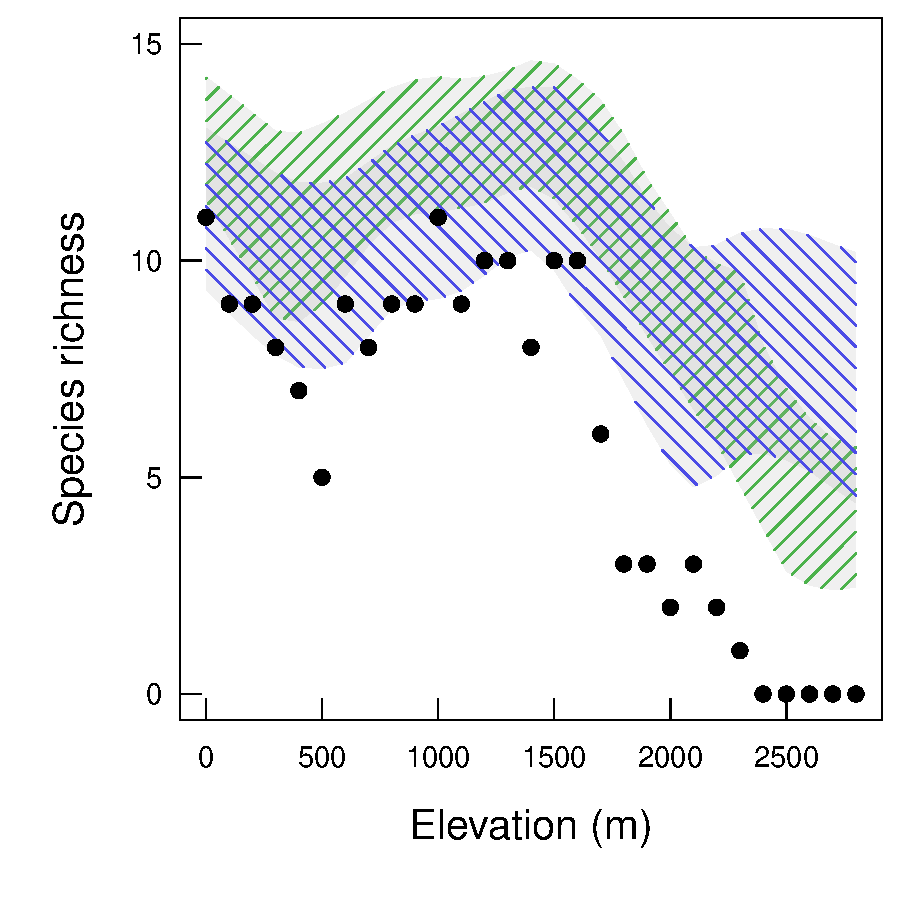
\includegraphics[width=0.5\linewidth]{../figures/div98-Sexonul-1} 

\end{tabular}
\caption{\label{fig:Snul}}
\end{figure}

\clearpage

\section{Tables}\label{tables}

\section{Supporting information}\label{supporting-information}

% latex.default(era, cdec = c(0, rep(0, 5)), caption = "Summary of species elevation patterns",      ctable = FALSE, label = "era", file = "tables/zoizos_era.tex") 
%
\begin{table}[!tbp]
\caption{Summary of species elevation patterns\label{tbl:era}} 
\begin{center}
\begin{tabular}{|lrrrrr|}
\toprule
\multicolumn{1}{|l}{Species}&\multicolumn{1}{c}{Occurrence}&\multicolumn{1}{c}{Mean (m)}&\multicolumn{1}{c}{Weighted mean (m)t}&\multicolumn{1}{c}{Min.}&\multicolumn{1}{c|}{Max.}\tabularnewline
\midrule
ACTR&$168$&$1084$&$1123$&$  20$&$2400$\tabularnewline
CIMA&$  6$&$1058$&$1049$&$ 800$&$1370$\tabularnewline
COCH&$  1$&$1010$&$1010$&$1010$&$1010$\tabularnewline
COCO&$ 33$&$1267$&$1307$&$ 320$&$1700$\tabularnewline
COFR&$ 57$&$1115$&$ 974$&$ 185$&$1660$\tabularnewline
ESAS&$ 88$&$1001$&$ 987$&$  60$&$1720$\tabularnewline
FOMA&$268$&$1051$&$1033$&$  20$&$2250$\tabularnewline
FRPO&$  2$&$ 128$&$ 142$&$  70$&$ 185$\tabularnewline
GEST&$109$&$ 840$&$ 804$&$  20$&$1620$\tabularnewline
HYBO&$ 67$&$1405$&$1410$&$ 620$&$2560$\tabularnewline
MAMA&$  5$&$1528$&$1615$&$1240$&$1705$\tabularnewline
PADO&$ 72$&$1128$&$1202$&$  65$&$1960$\tabularnewline
PEAS&$ 16$&$ 117$&$ 119$&$  50$&$ 290$\tabularnewline
PHBO&$  1$&$1495$&$1495$&$1495$&$1495$\tabularnewline
PLCU&$ 32$&$ 580$&$ 606$&$  65$&$1345$\tabularnewline
PYJO&$ 72$&$ 794$&$ 805$&$  65$&$1690$\tabularnewline
SATE&$202$&$1590$&$1601$&$ 270$&$2880$\tabularnewline
STPI&$ 34$&$1181$&$1225$&$ 100$&$2150$\tabularnewline
TEBO&$ 18$&$1307$&$1336$&$ 900$&$1680$\tabularnewline
TUNI&$ 41$&$ 832$&$ 808$&$  35$&$1700$\tabularnewline
ZOBO&$229$&$1371$&$1347$&$  60$&$2700$\tabularnewline
ZOOL&$ 45$&$1391$&$1388$&$ 620$&$2600$\tabularnewline
\bottomrule
\end{tabular}
\end{center}
\end{table}



\clearpage

\renewcommand{\thefigure}{S\arabic{figure}}

\setcounter{figure}{0}

\renewcommand{\thetable}{S\arabic{table}}

\setcounter{table}{0} \begin{table}
\caption{List of bird species detected in the study\label{tbl:species}}
\footnotesize
\begin{tabular}{|llllcccc|}
\toprule
\multicolumn{1}{|c}{\textbf{Label}}& \multicolumn{1}{c}{\textbf{Species}} & \multicolumn{1}{c}{\textbf{Order}} & \multicolumn{1}{c}{\textbf{Family}} & \textbf{Mass} (g) & \textbf{Size} (cm) & \textbf{Status} & \textbf{RLI} \\
\midrule
ACTR & Acridotheres tristis & Passeriformes & Sturnidae & 82 – 134 & 23 – 29 & E & LC \\ 
CIMA & Circus maillardi & Accipitriformes & Accipitridae & 50 & 650 – 1000 & R  & EN  \\
COFR & Collocalia francica & Apodiformes & Apodidae & 7 – 13,3 &  & M & NT \\
COCH & Coturnix chinensis & Galliformes & Phasianidae & 31 – 41 & 12 – 15 & E & LC \\
COCO & Coturnix coturnix & Galliformes & Phasianidae & 16 & 70 - 135 & E & LC \\ 
ESAS & Estrilda astrild & Passeriformes & Estrildidae & 7 – 8 & 10 & E & LC \\ 
FOMA & Foudia madagascariensis & Passeriformes & Ploceidae & 13 & 17 – 19 & E & LC \\ 
FRPO & Francolinus pondicerianus & Galliformes & Phasianidae & 200 - 340 & 30 - 32 & E & LC \\ 
GEST & Geopelia striata & Columbiformes & Columbidae &  & 20 & E & LC \\ 
HYBO & Hypsipetes borbonicus & Passeriformes & Pycnonotidae & 22 & 51 - 57 & R  & LC \\ 
%LOPU & Lonchura punctata & Passeriformes & Estrildidae & 11 & 12 – 15 & E & LC \\ 
MAMA & Margaroperdrix madagascariensis & Galliformes & Phasianidae &  & 24 - 26 & N & LC \\ 
PADO & Passer domesticus & Passeriformes & Passeridae & 26 - 32 & 14 - 16 & E & LC \\ 
PEAS & Perdicula asiatica & Galliformes & Phasianidae & 57 - 82 & 17 & N & LC \\ 
PHBO & Phedina borbonica & Passeriformes & Hirundinidae &  & 13,5 & E & LC \\ 
PLCU & Ploceus cucullatus & Passeriformes & Ploceidae & 17 & 32 – 45 & E & LC \\ 
PYJO & Pycnonotus jocosus & Passeriformes & Pycnonotidae & 20 & 23 – 42 & E & LC \\ 
SATE & Saxicola tectes & Passeriformes & Muscicapidae & 12,5 & 10,5 – 15 & R  & LC \\ 
STPI & Streptopelia picturata & Columbiformes & Columbidae & 28 & 145 – 255 & N & LC  \\ 
TEBO & Terpsiphone bourbonnensis bourb. & Passeriformes & Monarchidae & 15 & 10 – 12 & M (R)  & LC \\ 
TUNI & Turnix nigricollis & Turniciformes & Turnicidae &  & 13 & N & LC  \\ 
ZOBO & Zosterops borbonicus borbonicus & Passeriformes & Zosteropidae & 10 & 7 – 8 & M (R)  & LC \\ 
ZOOL & Zosterops olivaceus & Passeriformes & Zosteropidae & 10,5 & 9 – 10 & R  & LC \\ 
\bottomrule
\end{tabular}
\end{table}


%------- bibliography ----------------

\printbibliography



	
\end{document}
